% !Mode:: "TeX:UTF-8"
\documentclass{article}
% !Mode:: "TeX:UTF-8"
\usepackage[english]{babel}
\usepackage[UTF8]{ctex}
\usepackage{amsmath, amsthm, amssymb}

% Figure
\usepackage{graphicx}
\usepackage{float} %% H can fix the location
\usepackage{caption}
\usepackage[format=hang,singlelinecheck=0,font={sf,small},labelfont=bf]{subfig}
\usepackage[noabbrev]{cleveref}
\captionsetup[subfigure]{subrefformat=simple,labelformat=simple,listofformat=subsimple}
\renewcommand\thesubfigure{(\alph{subfigure})}

\usepackage{epstopdf} %% convert eps to pdf
\DeclareGraphicsExtensions{.eps,.mps,.pdf,.jpg,.png} %% bmp, gif not supported
\DeclareGraphicsRule{*}{eps}{*}{}
\graphicspath{{img/}{figure/}{../figure/}} %% fig directorys

%% \usepackage{pstricks} %% a set of macros that allow the inclusion of PostScript drawings directly inside TeX or LaTeX code
%% \usepackage{wrapfig} %% Wrapping text around figures

% Table
\usepackage{booktabs} %% allow the use of \toprule, \midrule, and \bottomrule
\usepackage{tabularx}
\usepackage{multirow}
\usepackage{colortbl}
\usepackage{longtable}
\usepackage{supertabular}

\usepackage[colorinlistoftodos]{todonotes}

% Geometry
\usepackage[paper=a4paper, top=1.5cm, bottom=1.5cm, left=1cm, right=1cm]{geometry}
%% \usepackage[paper=a4paper, top=2.54cm, bottom=2.54cm, left=3.18cm, right=3.18cm]{geometry} %% ms word
%% \usepackage[top=0.1cm, bottom=0.1cm, left=0.1cm, right=0.1cm, paperwidth=9cm, paperheight=11.7cm]{geometry} %% kindle

% Code
%% \usepackage{alltt} %% \textbf can be used in alltt, but not in verbatim

\usepackage{listings}
\lstset{
    backgroundcolor=\color{white},
    columns=flexible,
    breakatwhitespace=false,
    breaklines=true,
    captionpos=tt,
    frame=single, %% Frame: show a box around, possible values are: none|leftline|topline|bottomline|lines|single|shadowbox
    numbers=left, %% possible values are: left, right, none
    numbersep=5pt,
    showspaces=false,
    showstringspaces=false,
    showtabs=false,
    stepnumber=1, %% interval of lines to display the line number
    rulecolor=\color{black},
    tabsize=2,
    texcl=true,
    title=\lstname,
    escapeinside={\%*}{*)},
    extendedchars=false,
    mathescape=true,
    xleftmargin=3em,
    xrightmargin=3em,
    numberstyle=\color{gray},
    keywordstyle=\color{blue},
    commentstyle=\color{green},
    stringstyle=\color{red},
}

% Reference
%% \bibliographystyle{plain} % reference style

% Color
\usepackage[colorlinks, linkcolor=blue, anchorcolor=red, citecolor=green, CJKbookmarks=true]{hyperref}
\usepackage{color}
\def\red#1{\textcolor[rgb]{1.00,0.00,0.00}{#1}}
\newcommand\warning[1]{\red{#1}}

% Other
%% \usepackage{fixltx2e} %% for use of \textsubscript
%% \usepackage{dirtree}  %% directory structure, like the result of command tree in bash shell


% !Mode:: "TeX:UTF-8"
%+++++++++++++++++++++++++++++++++++article+++++++++++++++++++++++++++++++++
%customize the numbering of equation, to make it like section-subsection-equation style, for example,1-2-3
\makeatletter\@addtoreset{equation}{subsection}\makeatother
\renewcommand\theequation{%
\thepart\arabic{section}%
-\thepart\arabic{subsection}%
-\thepart\arabic{equation}%
}
%theorem
\newtheorem{definition}{D\'efintion} %% 整篇文章的全局编号
\newtheorem*{thmwn}{Thm} %% without numbers
\newtheorem{theorem}{Th\'eor\`eme}[section] %% 从属于section编号
\newtheorem{corollary}{Corollary}[theorem] %% 从属于theorem编号
\newtheorem{lemma}{Lemma}
\newtheorem{proposition}{Proposition}[section]
\newtheorem{example}{Example}
\newtheorem*{attention}{Attention}
\newtheorem*{note}{Note}
\newtheorem*{remark}{Remark}
\newtheorem{question}{Question}[section]
\newtheorem{problem}{Problem}
\newtheorem{fact}{Fact}


\begin{document}
\title{Optimisation}
\author{Common}
\maketitle
\newpage
\tableofcontents
\newpage

\section{拉格朗日乘数}
微积分中最常见的问题之一是求一个函数的极大极小值(极值).但是很多时候找到极值函数的显式表达是很困难的,特别是当函数有先决条件或约束时.
拉格朗日乘数则提供了一个非常便利方法来解决这类问题,而避开显式地引入约束和求解外部变量.

\subsection{Theory}
\begin{figure}[htbp]
  \centering
  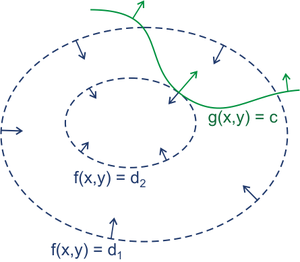
\includegraphics[scale = 0.5]{Lagrange_multiplier}\\
  \caption{Lagrange multiplier}\label{fig.Lagrange.multiplier}
\end{figure}

先看一个二维的例子:假设有函数:$f(x, y)$,要求其极值(最大值/最小值),且满足条件
$$ g\left( x,y \right) = c, $$
c 为常数.对不同$d_n$的值,不难想像出

$$ f \left( x, y \right)=d_n $$
的等高线, 如图\ref{fig.Lagrange.multiplier}, 
\href{http://upload.wikimedia.org/wikipedia/commons/thumb/f/fa/Lagrange\_multiplier.png/300px-Lagrange\_multiplier.png}{Lagrange multiplier}所示.
而方程 g 的可行集所构成的线正好是 $g ( x, y ) = c$ .想像我们沿着 $g = c$ 的可行集走,
因为大部分情况下 f 的等高线和 g 的可行集线不会重合,但在有解的情况下,这两条线会相交.想像此时我们移动 $g = c$ 上的点,因为 f 是连续的方程,
我们因此能走到$f \left( x, y \right)=d_n$更高或更低的等高线上,也就是说$d_n$可以变大或变小.只有当 $g = c$ 和$f \left( x, y \right)=d_n$相切,也就是说,
此时,我们正同时沿着 $g = c$ 和$f \left( x, y \right)=d_n$走.这种情况下,会出现极值或鞍点.

用向量的形式来表达的话,我们说相切的性质在此意味着 f 和 g 的切线在某点上平行.此时引入一个未知标量$\lambda$,并求解:

$$ \nabla \Big[f \left(x, y \right) + \lambda \left(g \left(x, y \right) - c \right) \Big] = 0 $$
且$\lambda \neq 0$.

一旦求出$\lambda$的值,将其套入下式,易求在无约束极值和极值所对应的点.

$$ F \left( x , y \right)  =  f \left( x , y \right) + \lambda \left( g \left( x , y \right) - c \right) $$
新方程$F(x,y)$在达到极值时与$f(x,y)$相等,因为$F(x,y)$达到极值时$g(x,y)-c$总等于零.

\subsection{Example}
\begin{example}
\textbf{求方程的最小值}:

$$ f(x, y) = x^2 y $$
同时未知数满足

$$ x^2 + y^2 = 1 $$
因为只有一个未知数的限制条件,我们只需要用一个乘数$\lambda$.

$$
\begin{aligned}
		& g (x, y) = x^2 +y^2 -1 \\
		& \Phi (x, y, \lambda) = f(x,y) + \lambda g(x, y) = x^2 y + \lambda (x^2 + y^2 - 1)
\end{aligned}
$$
将所有$\Phi$方程的偏微分设为零,得到一个方程组,最大值是以下方程组的解中的一个:

$$
\begin{aligned}
		& 2 x y + 2 \lambda x = 0 \\
		& x^2 + 2 \lambda y = 0 \\
		& x^2 + y^2 -1 = 0
\end{aligned}
$$
求解方程组,结果
\end{example}

\begin{example}
\textbf{离散分布的最大熵}:

$$ f(p_1,p_2,\ldots,p_n) = -\sum_{k=1}^n p_k\log_2 p_k.  $$
所有概率的总和是1,因此我们得到的约束是$g(p)= 1$即

$$ g(p_1,p_2,\ldots,p_n)=\sum_{k=1}^n p_k=1.  $$
可以使用拉格朗日乘数找到最高熵(概率的函数).对于所有的k 从1到n,要求

$$ \frac{\partial}{\partial p_k}(f+\lambda (g-1))=0, $$
由此得到

$$ \frac{\partial}{\partial p_k}\left(-\sum_{k=1}^n p_k \log_2 p_k + \lambda (\sum_{k=1}^n p_k - 1) \right) = 0.  $$
计算出这n个等式的微分,我们得到:

$$ -\left(\frac{1}{\ln 2}+\log_2 p_k \right) + \lambda = 0.  $$
这说明$p_i$都相等 (因为它们都只是$\lambda$的函数). 解出约束$\sum_k p_k = 1$,得到

$$ p_k = \frac{1}{n}.$$
因此,使用均匀分布可得到最大熵的值.
\end{example}
\end{document}
